\chapter{Problemanalyse}\label{chapter:problemanalyse}
I dette kapitel lægges rammerne for problemet fast.
Problemet som udforskes her, er problematikker i forhold til madlavning og indkøb i hverdagen. 

Først foretages en indledende interviewrunde der har til formål at bekræfte og klarlægge problemet, samt at undersøge om der er interesse for løsninger til problemet.
Efter dette foretages en analyse af state of the art, der har til formål at undersøge og udforske eksisterende løsninger til problemet.
Der skal altså undersøges hvilke funktionaliteter løsningerne har, samt om løsningerne er tilfredsstillende.
Efter denne undersøgelse, udføres endnu et interview.
Dette interview skal undersøge hvilke funktionaliteter potentielle brugere har interesse for, hvilket gøres i forbindelse med gruppens egen prototype.
Sidst i kapitlet defineres problemformuleringen, som danner grundlag for den resterende del af projektet.


\section{Indledende interview}
Onsdag d. 17 september gennemførte vi en række semi-strukturerede interviews i Aalborg midtby blandt folk omkring Føtex.
Vi adspurgte syv personer i forskellige målgrupper, herunder unge der bor alene, unge der bor sammen med nogen, og  folk over 30 med begge førnævnte sociale statusser.
Aldersspændet var fra 20 - 51, og kønnene var ligeligt fordelt.
Formålet med disse interviews var at danne et basalt overblik over vores problemområde, samt undersøge, hvordan folk håndterede vores initierende problem på nuværende tidspunkt.
Vores interviews bestod af en håndfuld forberedte spørgsmål, samt løsere samtale, for at følge op på disse spørgsmål.
Ud af interviewene fandt vi følgende hovedpunkter:
\begin{itemize}
	\item Generelt er folk uorganiserede når det kommer til indkøb, og især unge mennesker bruger sjældent indkøbslister.
	\item Inspiration til aftensmåltider findes ofte i indkøbssituationen eller ud fra princippet “hvad man lige har lyst til”.
	\item Det er ikke mange, der gennemgår tilbudsaviser, og endnu færre går bevidst efter tilbud.
	Dog kan det påvirke beslutninger om aftensmåltid, hvis en given varer er på tilbud i butikken, hvor der handles ind.
	\item Især den yngre målgruppe (18-28) er interesseret i en løsning med tilbud, indkøbslister og opskrifter til inspiration kædet sammen. Mens den ældre målgruppe (28+) virker mere interesseret i at kunne dele indkøbslister med familie, for bedre at kunne organisere indkøb.
	\item Opskrifter er som sagt noget, der mest interesserer det yngre segment.
	Dog påpeger nogle, at stor tendens til at være kræsen kræver at man kan sætte præferencer.
\end{itemize}

Dog skal det nævnes, at der bør evalueres over designet og funktionaliteterne med brugerne for at sikre et brugbart produkt til slut.
Fremadrettet vil der arbejdes videre med følgende områder:

\begin{itemize}
	\item Indkøbslister
	\item Tilbud
	\item Opskrifter.
\end{itemize}

\section{State of the art}\label{s:SOTA}
I dette afsnit har vi forsøgt at finde en bred vifte af forskellige løsninger der kan løse et eller flere problemer i forbindelse med indkøb og madlavning, omhandlende indkøbslister, tilbud og opskrifter.

Der vil blive kigget på web services og applikationer, der har til formål at løse nogle af de samme problemer, der berører vores emne.
Løsningerne, der er præsenteret i dette afsnit, forsøger at afhjælpe de problemer beskrevet af de adspurgte i interviewene i \myref{section:interview1}.

\subsection{eTilbudsavis}
eTilbudsavis er en online service, der kan findes på deres hjemmeside\footnote{\underline{www.etilbudsavis.dk}}. eTilbudsavis er en online avis med en høj funktionalitet og en nem brugergrænseflade.
Der kan på siden oprettes et login, således der kan findes tilbage til ændringer på et senere tidspunkt eller andre enheder.
eTilbudsavis har tre mærkbare funktioner, som brugeren har adgang til, hvilket er tilbudsaviser, ønske- og indkøbslister og tilbud.

Tilbudsavis-funktionen, hvilket kan ses på \myref{ss:eTilbudsavis}, indeholder også den mulighed at sætte en præference på, hvor stor en radius man vil lede i efter butikkers tilbudsaviser.
Under hver avis, som det ses på figuren, er der også angivet afstand i meter fra ens aktuelle placering.
Der kan vælges imellem alle aviser, som er tilgængelige online og inden for den valgte radius.
Aviserne bliver opdateret løbende, så når der er en ny tilgængelig, bliver den gamle fjernet.
Inde i aviserne kan man trykke på en tilbud, og denne tilføjes til en liste.

\begin{wrapfigure}{o}{0.68\textwidth}
\vspace{-20pt}
	\begin{center}
		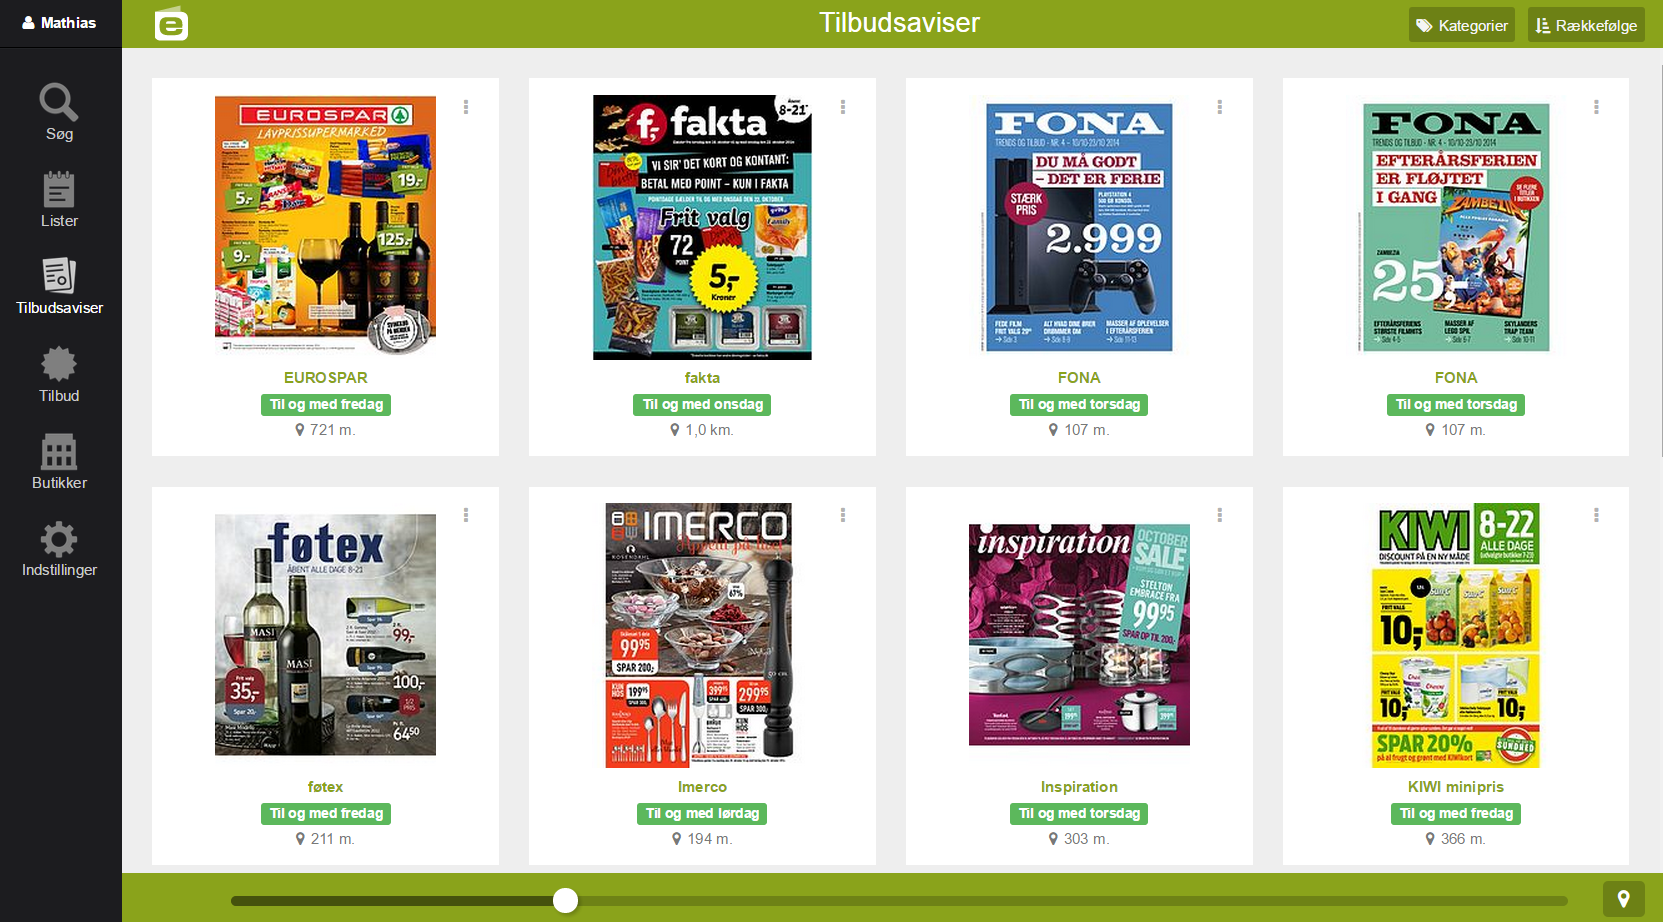
\includegraphics[width=0.66\textwidth]{images/Images/eTilbudsavis.PNG}
	\end{center}
	\vspace{-20pt}
	\caption{Tilbudsaviser på eTilbudsavis.dk}\label{ss:eTilbudsavis}
	\vspace{-20pt}
\end{wrapfigure}

Der er mulighed for at tilføje varer til to lister, en indkøbsliste og en ønskeliste.
Når en vare er valgt, bliver den tilføjet til den valgte liste.
Listen indeholder navn, butik, pris og den valgte mængde, for varen.
Der kan foruden det at vælge varer fra tilbudsaviserne, nemt skrives generiske varer på listen. Varen på listen kan da krydses af for at kunne holde styr på, hvad der er blevet købt.

Hvis der ikke ønskes at skulle bladres tilbudsaviser igennem, er der den mulighed at få vist en hel side kun med tilbud.
Alle aktuelle tilbud fra aviserne, er da vist som elementer med navn, beskrivelse, pris, butik og afstand. Disse tilbud kan på samme måde nemt tilføjes til listerne.

eTilbudsavis er en god online løsning, som har mange gode features, derfor har vi også brugt dem som kilde til vores tilbud gennem deres API.
Dette API er beskrevet i \myref{api}. \myref{Skal vi nævne det allerede her ?}

\subsection{Tilbudsugen}
Tilbudsugen minder på mange måder om eTilbudsavis, og kan findes på deres hjemmeside\footnote{\underline{www.tilbudsugen.dk}}.
Den har samtlige dagligvareaviser, samt flere inden for bl.a. byggemarkeder, og autoudstyr.
De giver et nemt overblik over diverse aviser, og man kan hurtigt og nemt læse dem på nettet.
Der er desuden mulighed for at lave præferencer som ved eTilbudsavis, her kan man bl.a. vælge økologi eller nøglehulsmærket.
Når man tilføjer en vare til indkøbslisten, søger den automatisk efter tilbud på den valgte vare.
Man bliver bedt om at vælge et specifikt tilbud, og netop dette tilbud bliver tilføjet til indkøbslisten med pris, butik, udløbsdato, mængde og et billede af varen.
Man kan som i eTilbudsavis også trykke på en vare direkte i avisen for at tilføje den til sin liste.
Hvis man vil dele sin indkøbsliste, er det også en mulighed vha. en ``delekode'' som man kan give til en anden bruger - de kan på denne måde også se listen.
Funktionerne findes på hjemmesiden, men det er ikke altid de virker.
For eksempel hvis man tilføjer noget uden at angive et antal, og du så prøver at dele listen med en, vil de ikke være at finde på listen.
Desuden kan man ikke ændre på antallet af varen, du allerede har sat på din indkøbsliste.
For at opnå dette, skal man slette varen, og tilføje den igen med det nye antal.
De har desuden også en smartphone app, men denne crasher ofte, når man benytter sig af deres indkøbsliste, men fungerer tilgengæld fint, hvis man blot vil se på ugens tilbud i aviserne.

Tilbudsugen er et lidt dårligere alternativt til eTilbudsavis, da der er problemer med delbarheden af indkøbslisterne, samt den app, der er stillet til rådighed, ikke er stabil.
Derimod er den nem at navigere, siden er brugervenlig og ser overskuelig ud.

\subsection{Smartphone Apps udgivet af butikker}
På \myref{tbl-smartphone} ses der nogle butikskæder, som har udviklet android apps, samt hvilke funktionaliteter disse har.
For at skabe et overblik, er der udvalgt features, og disse er blevet opsat i et skema for overskuelighedens skyld.
\begin{table}[H]
	\centering
		\colorlet{shadecolor}{gray!40}
    	\rowcolors{1}{white}{shadecolor}
	    \begin{tabular}{l|lllllllllll}
	    %Table: http://bit.ly/1tD6EI6
	   	%Funktionalitet & Tilbudsavis & Indkøbsliste & Opskrifter & Varescan & Find butik & Budget & Madplan & Rabatkupon/fordelsordning & Deling af indkøbslister & Rating på Play & Senest opdateret \\ \hline
	     & \rot{Tilbudsavis} & \rot{Indkøbsliste} & \rot{Opskrifter} & \rot{Varescan} & \rot{Find butik } & \rot{Budget} & \rot{Madplan} & \rot{Rabatkupon} & \rot{Deling} & \rot{Play rating} & \rot{Senest} \rot{opdateret} \\ \hline
	   	Føtex                       & \cmark   & \cmark    & \cmark  & \cmark   & \cmark  & ~      & ~       & ~          & ~                       & 3.4 (354)      & 2014-07-24       \\
	    SPAR                        & \cmark   & \cmark    & \cmark  & ~        & \cmark  & \cmark & ~       & ~          & ~                       & 2.8 (64)       & 2014-05-15       \\
	    Fakta                       & \cmark   & \cmark    & \cmark  & ~        & \cmark  & ~      & \cmark        & \cmark     & \cmark               & 3.1 (454)      & 2014-08-02       \\
	    FaktaQ                      & \cmark   & ~         & \cmark  & ~        & \cmark  & ~      & ~       & ~          & ~                       & 4.4 (7)        & 2014-03-11       \\
	    REMA 1000                   & \cmark   & \cmark    & \cmark  & ~        & \cmark  & ~      & ~       & ~          & ~                       & 3.5 (674)      & 2014-04-16       \\
	    SuperBrugsen                & \cmark   & \cmark    & \cmark  & ~        & \cmark  & ~      & ~       & ~          & ~                       & 3.8 (987)      & 2014-06-30       \\
	    Kvickly                     & \cmark   & \cmark    & \cmark  & ~        & \cmark  & ~      & ~       & ~          & ~                       & 3.7 (632)      & 2014-07-20       \\
	    \end{tabular}
	    \caption{Nogle butikskæder med smartphone apps samt deres funktionaliteter.}\label{tbl-smartphone}
	\end{table}
Vi har valgt at beskrive en af disse apps nærmere, og valget faldt på Faktas app, MitFakta, da denne bliver opdateret og har flest funktioner.
\subsubsection{Faktas Android App}

\begin{wrapfigure}{o}{0.4\textwidth}
\vspace{-20pt}
	\begin{center}
		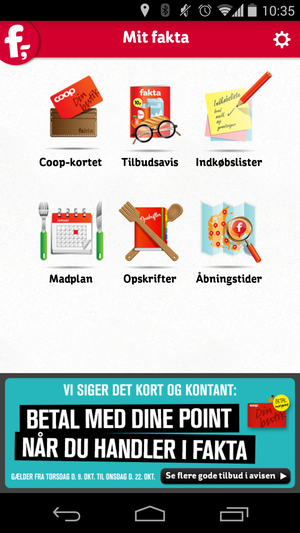
\includegraphics[width=0.38\textwidth]{images/Images/MitFakta.png}
	\end{center}
	\vspace{-20pt}
	\caption{MitFakta}
	\vspace{-20pt}
	\label{ss:MitFakta}
\end{wrapfigure}

Faktas android app er som helhed overskuelig.
Efter åbning af appen kan man vælge mellem seks menupunkter eller ændre sine indstillinger, disse kan ses på \myref{ss:MitFakta}.
Første menupunkt omhandler ``Coop-kortet'', og giver brugeren mulighed for at indtaste sine medlemsinfomationer, da disse giver særlige tilbud.
Andet menupunkt er deres tilbudsavis, hvilket er en digital kopi af den fysiske tilbudsavis.
Dog kan man fra den også tilføje varer til sin indkøbsliste, eller se varerne i et gitterformat.
Tredje menupunkt er ``indkøbsliste'', her kan man have flere personlige og/eller delte indkøbslister.
Her kommer deres Facebook integration også i spil, som tillader nem deling af indkøbslister med brugerens Facebook venner.
Fjerde menupunkt er en madplan, hvori man kan planlægge sin egen madplan, eller se Faktas anbefalinger til en ``under 20 kr pr. person pr. aften''-løsning.
Femte menupunkt er deres opskrifter.
Her findes der et stort antal af opskrifter, disse kan tilføjes direkte til ens madplan eller indkøbslister (både personlige og delte).
Sjette menupunkt hedder ``Åbningstider'', og her kan brugeren finde Faktas butikker samt deres forskellige åbningstider.

Appen virker rigtig godt, der er ingen blindgyder, og derfor er den meget nem at navigere rundt i. Der er lagt megetxnote{Meget alligevel?} fokus på den sociale del, da der kan deles med venner på facebook, hvilket simplificerer delingen af indkøbslister. Den eneste ulempe, der er ved denne app, er, at den kun er egnet til vare fra Fakta, og derfor sætter en del restriktioner på sig selv.

\subsection{Tøm køleskabet} \fxnote{Er dette afsnit relevant længere, vi bruger det jo ikke senere? - Troels Jeg tænker vi kan prøve at bruge det senere, vi afgrænser os vel fra at lave lagerstyrring eller tøm køleskabet, det var nok tanken at det var det vi ville da dette blev skrevet? - Søren}
Der findes talrige tjenester, der tilbyder ``at tømme dit køleskab''.
Mere specifikt, tilbyder de en service, hvor du som bruger, angiver hvilke varer dit køleskab pt. indeholder, samt hvilke andre ingredienser du har til rådighed.
Derefter får du så præsenteret en række forskellige opskrifter, der kan laves ud fra dine tilgængelige ingredienser.
De fleste af tjenesterne (herunder dem vi her har undersøgt) viser også opskrifter, som indeholder yderligere ingredienser.
Dette betyder naturligvis, at man som bruger ikke bliver fritaget fra at handle ind, hvis man mangler nogle ingredienser til lige netop den opskrift, man vælger at udføre.
Tjenesten \textit{MyFridgeFood} \footnote{\underline{www.myfridgefood.com}} tilbyder at oprette en indkøbsliste ud fra netop disse manglende ingredienser, hvilket kan lade sig gøre blandt andet fordi, alle opskrifter er interne på \textit{MyFridgeFood}.
I modsætning til dette er der \textit{Supercook} \footnote{\underline{www.supercook.com}}, som linker til eksterne opskrifter, og ikke tilbyder at generere en indkøbsliste.
Umiddelbart anbefales opskrifter ikke ud fra den enkelte brugers smag og madvaner, men udelukkende på baggrund af, hvad man ``har i køleskabet''.
Grundet dette virker tjenesterne mere som simple filtreringer af databaseopslag, end egentlige anbefalinger, der tager højde for brugerens smag og præferencer indenfor den gastronomiske verden.

Som vi har set i ovenstående gennemgang, findes der alternativer til den klassiske indkøbstur, der er dog ingen af disse, der formår at løse alle problemerne.
Ved alle løsningerne opstår også nye ulemper og problemstillinger i forhold til almindeligt indkøb.
Alt taget i betragtning vil det komme meget an på nuværende vaner og familiestrukturen, om disse muligheder vil være en god løsning for en given familie.

\section{Prototype interviews}\label{section:interview2}
State of The Art undersøgelsen viste at der er mange forskellige løsninger, men der er også mange mangler i disse alligevel.
Ingen af løsningerne tager tilbud fra alle butikker, har indkøbsliste, tilbyder opskrifter der er integreret med tilbudene, samt vurdering af disse.
Løsningerne
Derfor har vi udformet en prototype i Microsoft Office Powerpoint som viser forskellige funktionaliteter.
Diasshowet består af forskellige skærmbilleder, som der kan navigeres imellem ved tryk på de gule felter.

Et eksempel kan ses på \myref{ss:Prototype}.

\begin{wrapfigure}{o}{0.68\textwidth}
\vspace{-20pt}
	\begin{center}
		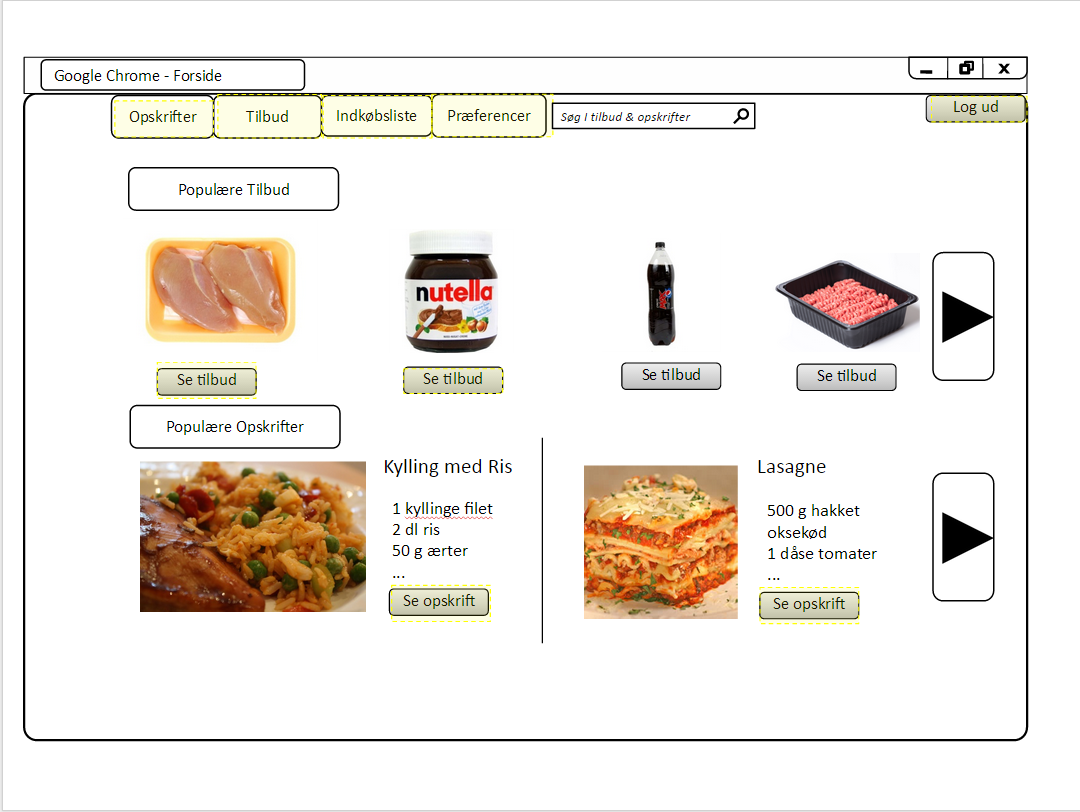
\includegraphics[width=0.66\textwidth]{images/Images/prototype-forside.PNG}
	\end{center}
	\vspace{-20pt}
	\caption{Forside fra Prototypen, der blev brugt i forbindelse med vores 2. runde af interviews}\label{ss:Prototype}
	\vspace{-20pt}
\end{wrapfigure}

Prototypen bruges i vores 2. runde af interviews, som har til formål at forstå hvilke funktionaliteter potentielle brugere ønsker i en løsning.
De interviewede bestod mest af unge personer i starten af tyverne, hvor af de fleste var studerende.
Dette valg blev taget da ud fra det første interview, hvor den primære interesse lå hos de unge, der i forvejen brugte deres smartphone og computer til planlægning af indkøb og aftensmad.
Således ville en overgang til en ny løsning her være mere naturlig end de ældre grupper, der ofte laver listen på papir og har bøger med opskrifter til at finde inspiration.
På trods af dette var der stadig en interesse i den ældre gruppe, og målgruppen er som følge deraf ikke udelukkende unge.

Den 2. runde af interviews blev udført som semi-struktureret interviews, med personer hvor der var oprettet kontakt på forhånd, frem for at finde fremmed på gaden.
Dette tillod os at interviewe i længere tid, såvel som at de interviewede i forvejen var forberedt på et interview.
Et semi-struktureret interview tillader at der afviges fra de nedskrevne spørgsmål, for at følge samtalen og stille uddybende spørgsmål omkring potentielle kommentare.\fxnote{Find eventuel kilde fra DEB? - Marc}

De spørgsmål, som de adspurgte blev præsenteret for, var lavet med den præmis at få deres tanker omkring et system, inden de blev repræsenteret for de idéer der ellers var omkring systemet.
For at opnå dette, blev de først spurgt om et spørgsmål som hvilke opgaver de mente systemet kunne behjælpe, hvorefter der blev uddybet hvorfor præcis disse funktionaliteter blev nævnt af de interviewede.
Først efter at have fået deres idéer, blev de repræsenteret for idéer projektgruppen havde opnået, og herefter reflekteret over hvorfor nogle ikke var nævnt, smat hvad de mente om disse forslag.
Et dokument over de strukturerede spørgsmål af interview-sessionerne, kan findes på \myref{}%Interview2

Ud fra den respons der blev opnået igennem undersøgelsen, står det klart at en løsning skal have følgende funktionaliteter:

\begin{itemize}
	\item Indkøbsliste integreret med tilbud.
	\item Oversigt over tilbud fra samtlige dagligvarebutikker.
	\item Opskrifter, som gør brug af tilbud.
	\item Mulighed for at vurdere opskrifterne og få anbefalet lignende.
	\item Valg af hvor man vil handle, hvilke madvarer man ikke vil spise osv.
	\item Deling af indkøbsliste med andre.
	\item Filtrering under opskrifter, så man kan se hvad man kan lave ud af f.eks. oksekød osv.
	\item Overvågning af varer, så man får en form for besked hvis noget kommer på tilbud en uge.
\end{itemize}

Der var også andre funktionaliteter som nogle af de adspurgte foreslog kunne laves for systemet, disse er dog blevet fravalgt, enten fordi det kun var enkelte der bakkede op omkring den funktion, eller at det ikke passede ind med systemets anden funktionalitet.
F.eks. blev en kalorietæller foreslået af en af de adspurgte, men dette vælges der at afgrænses fra, da det ikke hænger så godt sammen med resten af den meget tilbudsorienterede løsning.

Herudover gav de interviewende også forslag og råd angående hvilke funktionaliteter skulle være hvor i et desktop layout.
Disse forslag tages med i overvejelserne når brugergrænsefladen skal designes.
En oversigt over de adspurgtes svar såvel som forslag, kan ses på \myref{}%Interview2 Opsummering

\section{Problemformulering}\label{section:problemformulering}

I state of the art undersøgelsen \myref{s:SOTA} blev der undersøgt eksisterende løsninger, på problemet beskrevet i indledningen af rapporten. 
Der blev ikke fundet nogle løsninger, som løste alle de problemstillinger fundet i den første interviewrunde, og det blev desuden også klart, at ingen af de adspurgte fra første interviewrunde i \myref{section:interview1} brugte disse programmer.

Den viste samtidigt, at de interviewede havde en interesse for en software løsning på dette problem, hvis den havde features de andre programmer ikke har. 

I prototype interviewene blev vores Powerpoint prototype fremvist og testet, her blev flere funktionaliteter, som kunne inkluderes i systemet, udforsket.
Disse informationer har ledt til følgende problemstilling:

\[
  \left[
  \begin{minipage}{\textwidth}
  \centering
  \begin{minipage}{0.96\textwidth}
  Hvordan designes og implementeres et system, i C\#, der kan give brugere lettere adgang til dagligvarebutikkernes tilbud integreret med indkøbslister og opskrifter imens det gøres mere overskueligt, at handle ind til aftensmad?
  \end{minipage} 
  \end{minipage}                           
    \right]
\]
